\documentclass[12pt,a4paper]{article}
\usepackage[latin2]{inputenc}
\usepackage{graphicx}
\usepackage{ulem}
\usepackage{amsmath}
\begin{document}
Securing Distributed .NET Applications Using Advanced Runtime Access 
Control

Kriszti�n P�cza, Mih�ly Bicz�, Zolt�n Porkol�b

E�tv�s Lor�nd University, Fac. of Informatics, Dept. of Programming 
Lang. and Compilers, P�zm�ny P�ter s�t�ny 1/c. H-1117, Budapest, Hungary

kpocza@kpocza.net, mihaly.biczo@t-online.hu, gsd@elte.hu

\textbf{Abstract.} The architecture and integration of distributed 
applications increased in complexity over the last decades. It was 
Service Oriented Architecture (SOA) that answered most of the emerging 
questions by its explicit and contract-based interface definitions for 
services and autonomous components. The exposed functionality can be 
used by anyone who has access to the public interface of SOA 
applications. Due to loose security handling, risks often emerge in SOA 
applications. Interfaces are usually published to an unnecessarily wide 
set of clients. Although there are attempts to implement fine-grained 
access control mechanisms in object-oriented programming languages like 
Eiffel, C\# and Java, these solutions are in-process that means that 
they cannot cross service contract boundaries in distributed 
applications. For these, it is of utmost importance to validate the type 
and the identity of the caller, track the state of the business process 
and even validate the client itself using simple, declarative syntax. In 
this paper we present a framework that aims to introduce fine-grained 
access control mechanisms in the context of distributed .NET 
applications. We present a semi-formalized description of the framework 
and also a pilot implementation on the .NET platform.

\section{1 Introduction}
The complexity of IT systems has been getting increasingly complex ever 
since the beginning of software development. IT systems and the business 
processes they serve span over multiple networks, computers, and 
programming languages as well. What makes things even more complicated 
is that pieces of software serving specific business goals (the steps of 
business processes) are dynamically changing. As a consequence, 
architects and developers face system integration issues in a 
dynamically changing technical and business environment. Until recently, 
integration of systems has been performed either manually or using 
hard-coded modules that were difficult to maintain and failed in a 
changing environment. Manual integration has been time consuming and 
prone to errors, while hard coded solutions require knowledge of all 
connected systems and have to be re-designed and implemented when any of 
the underlying systems or steps of the business process changes.

It is Service Oriented Architecture (SOA) $[$1, 10$]$\textbf{ }that 
answers the most common difficulties of system integration. From the 
historical point of view, SOA is an evolution of modular programming, so 
it extends its basic principles. Reuse, granularity, modularity, 
composability, componentization, and interoperability are common 
requests for a SOA application as well as for modular object oriented 
applications. 

However, while the elementary building block of an object oriented 
software is the class, the basic element of a SOA application is 
typically a much larger component. These larger chunks of functionality 
are called services, and this is where the name Service Oriented 
Architecture originates from. Services implement a relatively large set 
of functionality, and should be as independent of each other as 
possible. This means that services should have control over the logic 
they encapsulate and should not call each other directly. Rather, if a 
more complex behavior is required, they should be composed to more 
complex composite services. In other words, services should be 
autonomous and composable.

Services expose their functionality through service contracts. A 
contract describes the functions that can be invoked, the communication 
protocols as well as the authentication and authorization schemes. The 
exposed functionality is usually a public interface that can be called 
by anyone who is authenticated, is aware of the existence of the service 
and uses the required communication protocol. The keyword is that the 
exposed functionality is basically \textit{public}, and users have 
quite limited amount of control over the identity and the nature of a 
caller. 

However, in a realistic scenario it can also happen that the identity of 
the caller or the set of allowed methods depends on the state of the 
underlying business process or other available information. This is 
usually hard to express, and due to the lack of technology support for 
fine-grained, or higher level access control, it is challenging to 
implement the above mentioned scenario using standard protocols, 
programming environments and tools.

In $[$4, 15$]$ we have implemented a pilot approach to implement 
Eiffel-like selective feature export in C\# 3.0. This solution makes it 
possible to control access to protected resources (methods of 'public' 
interfaces) in a declarative way using simple declarative syntax using 
the concepts of Aspect Oriented Programming $[$12$]$. Although the 
approach works well in everyday application, it cannot be applied in the 
case of distributed systems. 

What makes things even more complicated is that SOA usually integrates 
systems running on multiple computers and environments, in other words 
these systems are distributed ones. To successfully implement our 
solution we have to sacrifice the interoperability property of SOA, 
which means that our connected applications have to be created using 
homogeneous communication platforms. The exposed services are required 
to be aware of some information about clients. Although this requirement 
is not common for SOA applications, however, other important properties 
of SOA can remain unchanged (contract based interface specification, 
autonomous services). Moreover, the security validation attributes can 
be regarded as part of the contract.

In this paper our aim is to establish a framework that enables users to 
control access to the members of public interfaces in a SOA-enabled 
distributed object system $[$17$]$. 

 In Section 2 we present a simple motivating example that draws attention 
to issues when not using fine-grained access control mechanisms.

In Section 3 we present a semi-formalized approach to solving problems 
presented through the motivating example.

In Section 4 a possible implementation of the theory will be shown. The 
chosen environment is the .NET platform, the Workflow Foundation engine 
(now part of the .NET framework), and the C\# programming language. 

In Section 5 we show some related work and compare our solution to 
existing ones. In the closing section we summarize our results, and 
present further research areas. 

\section{2 Motivating Example}
\subsection{2.1 Ping-Pong Game}
In order to highlight the problematic parts when accessing fully public 
SOA interfaces, in this subsection we are going to show a simple 
motivating example. The example is a simple game, through which we 
describe distributed applications, public interfaces, and access control 
problems. 

First, we place the game in the previously described context. The 
players of the game run on different computers, so the game is a 
distributed application. Let's consider a very simple example: a 
ping-pong game. In each game there are two players who pass a ball to 
each other. The players register themselves at the game manager, who 
gives a unique identifier to each player. The game cannot start until 
there are exactly two players. The first registered player begins the 
game, in other words he passes the ball to the other player. The second 
player should not be allowed to handle the ball until the first player 
passes it to him. Once the ball is passed to the second player, it is 
his turn: now the first player should be denied to handle the ball until 
the second player passes it back, and so on.

The methods of the game are published as an interface. The Game manager 
class implements this interface and exposes methods of the game to 
possible clients, primarily players. 

The 'rules' of the game can be described as a workflow. The workflow 
itself and its state transitions is a finite state automaton. The finite 
state automaton can be described as a UML activity diagram $[$19$]$. The 
activity diagram can be seen in . In , the simplified class diagram of 
the ping-pong game can be seen.

\begin{figure}[h]
\centering
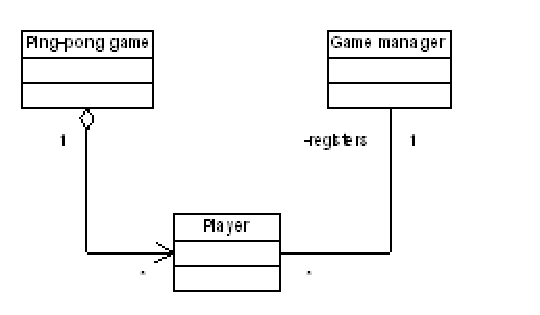
\includegraphics[width=253.05pt,height=141.3pt]{media/image1.eps}
\end{figure}
 



\begin{center}\textbf{Fig. 1. }Class diagram of ping-pong game
\end{center}

The game manager is a singleton, there is exactly one instance of the 
game manager class. Players register themselves at the game manager and 
get a unique identifier. A game manager can manage many games, and in 
each game there are exactly two players. Of course a game can be started 
only if there are exactly two players.

A possible object diagram can be seen in .



\begin{figure}[h]
\centering
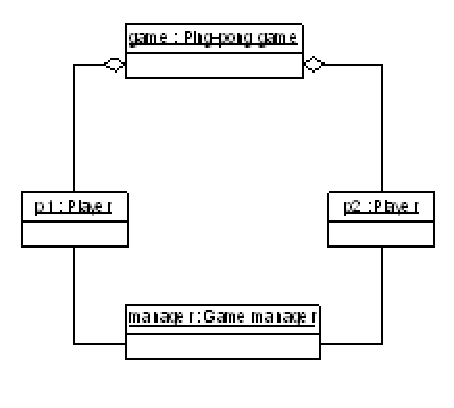
\includegraphics[width=213.3pt,height=190.2pt]{media/image2.eps}
\end{figure}


\begin{center}\textbf{Fig. 2. } Possible object diagram of a 
distributed game\end{center}



The objects may possibly run on different computers. The difficulty is 
that we want to allow only objects of type Player to call methods of the 
Ping-pong game object in this distributed environment. What makes things 
even more complicated is that the ping-pong game has a well-defined 
sequence of allowed events with a well-defined set of allowed callers, 
and we have to keep the system consistent based on these rules.

\subsection{2.2 Security Shortcomings of Recent Business Applications}
In real world business applications the sequence and branches of 
business operations that instrument business processes are well defined 
and bounded. It is also well defined who can execute a business 
operation in the lifetime of a business process instance.

The business rules clearly define who is allowed to perform different 
tasks and also define the exact workflow of our ping-pong game 
introduced before (even it is not a business application).

Unfortunately, in most real world applications these business rules are 
not enforced carefully on the server side, they are rather hard coded in 
the client application. Moreover, the restricted functions - based on 
the user role and the current state of the process - are simply hidden 
on the user interface. At the same time the server is open for any kind 
of requests, therefore an attacker can compromise the business process.



The reason of the previous can be one of the following:

\newcounter{numberedCntG}
\begin{enumerate}
\item Architects and developers do not care of business security
\item Architects and developers think that a simple firewall (that 
restricts the access of the server from specific subnets) or some 
built-in authentication is enough
\item Architects and developers think or decide that it is satisfying to 
implement business security on the client side
\item There is no time and money to implement adequate security 
mechanisms
\item It is hard to implement business security in a distributed 
environment
\setcounter{numberedCntG}{\theenumi}
\end{enumerate}
Of course it is hard or cannot be carried out to change the mind of 
architects and developers therefore we suggest a solution that makes 
server-side business security checks easier and faster to implement.

\section{3 Solve Shortcomings}
First we have to denote which client and business properties are 
suggested to be checked and tracked to raise the business process 
security level:

\newcounter{numberedCntH}
\begin{enumerate}
\item The runtime type of the caller class on the client side (ping-pong 
player in the ping-pong game)
\item State of the business process (e.g. The rules of the ping-pong 
game in our example)
\item The identity of the client (e.g. Is it the first or the second 
player in the ping-pong game?)
\item Validate, verify the client itself (e.g. IP address, subnet or 
some kind of certification of the client)
\setcounter{numberedCntH}{\theenumi}
\end{enumerate}
All of the previous are static or internal properties from the view of 
the business process, therefore all of them can be checked using 
\textit{declarative syntax} (statically burned in) or can be read from 
a configuration database. 

When creating a SOA application we publish a contract (an interface) to 
the outside world. The previous properties can be validated 
contract-wide and can be validated only for particular business 
operations published by the contract. 

It means that the above properties can be validated at method level at 
every single call. The granularity level of most of the above properties 
changes from application level to method level. Informally speaking we 
introduce a business call level fine-grained "\,firewall".

In the next subsections we will examine these four properties from the 
validability point of view.

We identified the need to give a semi-formalized description of our 
solution. There are two approaches:

\newcounter{numberedCntBD}
\begin{enumerate}
\item Extend some existing description language like BPEL $[$20, 11$]$
\item Create a new language that only focuses on the problem presented 
in this article
\setcounter{numberedCntBD}{\theenumi}
\end{enumerate}
Because BPEL focuses on the business process rather than security, and 
uses XML notation, we have chosen the second approach. BPEL and our 
semi-formal description can be used side-by-side.

A contract (C) can be defined as a triplet of set of methods, 
restrictions applied to the contract itself and the set of restrictions 
applied to individual methods published by the contract.

$C=(\lbrace M_{1},M_{2},\ldots ,M_{n}\rbrace , R_{C},\lbrace 
R_{M_{1}},R_{M_{2}},\ldots ,R_{M_{n}}\rbrace )$\\




The restrictions applied to the contract itself ($R_{c}$) can be 
formalized using the following triplet:

$R_{c}=(\lbrace T_{c_{1}},T_{c_{2}},\ldots ,T_{c_{q}}\rbrace ,\lbrace 
I_{c_{1}},I_{c_{2}},\ldots ,I_{c_{w}}\rbrace , \lbrace 
N_{c_{1}},N_{c_{2}},\ldots ,N_{c_{e}}\rbrace )$\\




Here $T_{c_{i}}$s represents a contract-level type restrictions for 
allowed callers (subsection 3.1), $I_{c_{i}}$s denotes a 
contract-level identity restrictions for allowed callers (subsection 
3.3), while $N_{c_{i}}$s defines a contract-level network restriction 
(subsection 3.4).

Security restrictions applied to a single method ($M_{i}$):



\begin{center}$R_{M_{i}}=(\lbrace T_{M_{i},1},T_{M_{i},2},\ldots 
,T_{M_{i},r_{i}}\rbrace ,\lbrace 
(S_{M_{i},1},A_{M_{i},1}),(S_{M_{i},2},A_{M_{i},2}),\ldots 
,(S_{M_{i},t_{i}},A_{M_{i},t_{i}})\rbrace ,$\\
\end{center}

\begin{center}$\lbrace I_{M_{i},1},I_{M_{i},2},\ldots 
,I_{M_{i},y_{i}}\rbrace ,\lbrace N_{M_{i},1},N_{M_{i},2},\ldots 
,N_{M_{i},u_{i}}\rbrace )$\\
\end{center}

Here $T_{M_{i},i}$s, $I_{M_{i},j}$s and $N_{M_{i},j}$s are the 
same as their contract-level pairs, while$ S_{M_{i},j},A_{M_{i},j}$ 
pairs describe the allowed state and state transition constraints 
(subsection 3.2).

\subsection{3.1 Distributed Runtime Access Control}
We have stated in one of our previous work about in-process systems 
$[$4$]$ that reducing the interface where software components can 
communicate with each other increases software quality, security and 
decreases development cost. Compile time or runtime visibility and 
access control checking that support encapsulation is the key part of 
modern languages and runtime environments $[$16$]$. They enforce 
responsibility separation, implementation and security policies. Most 
modern programming languages like C++, C\# and Java do not have 
sophisticated access control mechanisms only introduce a subset or 
combination of the following access modifiers: public, private, 
protected, internal, and friend while Eiffel defines sophisticated 
selective access control called selective export.

The Eiffel programming language $[$13$]$ allows features (methods) to be 
exposed to any named class. The default access level of a feature is the 
public level. However, an export clause can be defined for any feature 
which explicitly list classes that are allowed to access the underlying 
feature.

In this paper we suggest a runtime access control extension to 
distributed environments where only well identified classes are allowed 
to access particular methods. To achieve this goal, the server side 
should be extended with the ability to detect the runtime type of the 
caller (client) using a \textit{declarative solution} that statically 
predefines the allowed callers at the contract or method level.

Another possibility is to restrict access for clients based on group 
membership or roles (like DCOM $[$9$]$). In this case different callers 
in different roles are to be assigned to (domain level) groups and 
restrict access of published contracts for certain groups. Moreover, 
restrictions can be enforced at the operation (method) level to achieve 
more fine-grained security.

In our ping-ping example only players can participate in matches).

\subsection{3.2 Business Process Validation}
In $[$6$]$ it is noted that it may be necessary to impose constraints on 
who can perform a task given that a prior task has been performed by a 
particular individual. In this section we feature another approach to 
solve the problems stated in $[$6$]$.

As we mentioned before business applications are driven by rules that 
define the following properties:

\newcounter{numberedCntI}
\begin{enumerate}
\item Who is allowed to perform specific actions in given states
\item What is the resulting state of a state transition if a business 
operation succeeds
\item What is the resulting state of a state transition if a business 
operation fails
\setcounter{numberedCntI}{\theenumi}
\end{enumerate}
In most cases, business processes defined by rules are hard-coded into 
applications, therefore they can be treated as static properties.

As suggested before operations exported on the interface are statically 
bounded to certain process states in which they can be executed, 
furthermore often initiate a state transition where the process gets 
into another well-defined state.

Business processes can be represented by state machines which are a kind 
of directed graphs. Vertices of such a graph are the states of the state 
machine, while edges are the state transitions between states.

The state machine representing the 'business process' behind our 
ping-pong game can be described by the following UML Activity diagram in 
\textit{.} For the sake of simplicity we have not incorporated the 
error states and events where for example one of the players loses the 
ball.





\begin{figure}[h]
\centering
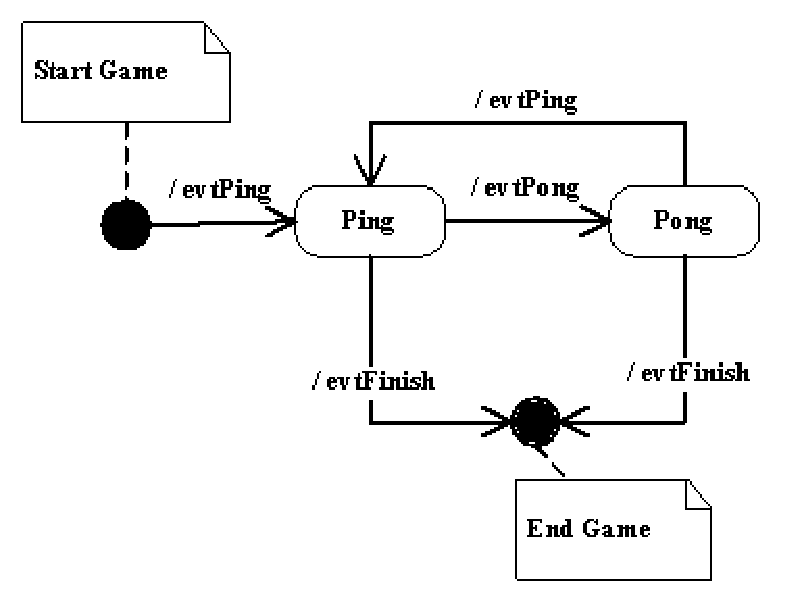
\includegraphics[width=193.45pt,height=146.15pt]{media/image3.eps}
\end{figure}


\begin{center}\textbf{Fig. 3. }State Machine of the ping-pong game
\end{center}



The first operation is where the first player gets the ball and hits it 
(\textit{evtPing}) to the other player therefore the game will be in 
\textit{Ping} state. After that the second player hits the ball (
\textit{evtPong}) to the first player and the game gets into \textit{
Pong} state. Now the first player comes again (\textit{evtPing}). 
If any of the players get bored of the game the match can be finished (
\textit{evtFinish}).

Manifestly, such state machines can be statically connected or bounded 
to one or more published contracts. Operations can be checked if the 
state machine is in a state that allows the particular operation and can 
trigger state transitions. When the user instantiates one of the 
published contracts a state machine instance is automatically attached 
to the contracts.

Static binding can be implemented declaratively and it is compulsory to 
have one state machine instance per session.

To describe it formally remind the definition of the finite state 
machine or simply state machine:



$FSM=(\Sigma ,S,s_{0},\delta ,F)$\\




Where 

\newcounter{numberedCntBA}
\begin{enumerate}
\item $\Sigma $ represents the input alphabet, in our case the set of 
state transitions
\item $S$ is a finite not empty set of states
\item $s_{0}$ is an initial state, that is member of S
\item $\delta : S\times \Sigma \to S$ is the state transition function 

\item F is the set of finite states, non-empty set in our case
\setcounter{numberedCntBA}{\theenumi}
\end{enumerate}


Using the above definition the following restrictions can be applied:



$\forall i\varepsilon \lbrack 1..n\rbrack :\forall j\varepsilon \lbrack 
1..t_{i}\rbrack \bigg\{ 
\begin{gathered}
S_{M_{i},j}\varepsilon S \\
A_{M_{i},j}\varepsilon \Sigma \\
(S_{M_{i},j},A_{M_{i},j})\varepsilon D_{\delta } \\
\end{gathered}
$\\
\\


It restricts the states, the state transitions and the state transitions 
available in certain states.

\subsection{3.3 Client Identity Validation}
In the previous two subsections we have shown that it is indispensable 
to restrict callers by runtime type or group membership and it is also 
indispensable to instrument the correct order of business operation 
execution, enforce business rules.

Notwithstanding the previously mentioned two assurances there is another 
problem that we show in the context of our ping-pong game. When Player 1 
and Player 2 start playing a ping-pong match we have to ensure that the 
players remain the same until the end of the match. In other words, they 
do not change sides and they are not substituted with other players. In 
short we have to maintain and validate the identity of players until the 
end of the match.

It is possible to dedicate a referee or coordinator that assigns 
well-defined identities for participants that can be ensured at method 
calls. For example the player that gets elected as First Player always 
gets Identity no. \textit{1} while the other player gets \textit{2}
.

The above may not give protection from tampering the player identity. 
But when we assign the \textit{(Name of the Computer, Process Id, 
Object Reference Id)} triplet to the identity and track it on the 
server side, it cannot be tampered because the name of the computer must 
be unique on the network level. Similarly the process id must be unique 
on the computer level; while the object reference id (practically pair 
of the runtime type and some type-level unique object id) must be unique 
on the process level (e.g. hash code is unique for same-typed objects in 
.NET).

\subsection{3.4 Network and Certificate Validation of Clients}
Firewalls can restrict access from clients deployed on certain subnets 
or IP addresses to the server. More advanced firewalls can restrict 
access to the server by domain level user identity; however that 
capability is only a subset of distributed runtime access control 
described in this paper.

Our first aim is to declaratively restrict access to specific contracts 
and also methods for certain subnets even IP addresses.

The other thing that loosely relates to some sort of network-level 
validation of clients is client certificate validation. Using client 
certificates it can be verified if the server communicates with a 
certified, trusted, verified and possibly well-working client. The 
server can verify if it communicates with clients having the certificate 
issued by a trusted authority.

\subsection{3.5 Definition of Legal Calls}
Let H the information-set provided and available at a method call:



\begin{center}$H=(T_{H},S_{a},I_{H},N_{H})$\\
\end{center}



Where

\newcounter{numberedCntBB}
\begin{enumerate}
\item $T_{H}$ is the type of the caller
\item $S_{a}$ the actual state (business process state)
\item $I_{H}$ is the identity of the caller
\item $N_{H}$ is the network properties of the caller
\setcounter{numberedCntBB}{\theenumi}
\end{enumerate}


We say that a call is legal with respect to a method ($M_{i}$), when 
H conforms to the following restrictions:



\newcounter{numberedCntBC}
\begin{enumerate}
\item $T_{H}\varepsilon \lbrace T_{M_{i},1},T_{M_{i},2},\ldots 
,T_{M_{i},r_{i}}\rbrace \bigcap{\lbrace T_{c_{1}},T_{c_{2}},\ldots 
,T_{c_{q}}\rbrace }$
\item $S_{a} \varepsilon \lbrace S_{M_{i},1},S_{M_{i},2},\ldots 
,S_{M_{i},t_{i}}\rbrace $
\item $I_{H}\varepsilon \lbrace I_{M_{i},1},I_{M_{i},2},\ldots 
,I_{M_{i},y_{i}}\rbrace \bigcap{\lbrace I_{c_{1}},I_{c_{2}},\ldots 
,I_{c_{w}}\rbrace }$
\item $N_{H}\varepsilon \lbrace N_{M_{i},1},N_{M_{i},2},\ldots 
,N_{M_{i},u_{i}}\rbrace \bigcap{\lbrace N_{c_{1}},N_{c_{2}},\ldots 
,N_{c_{e}}\rbrace }$
\setcounter{numberedCntBC}{\theenumi}
\end{enumerate}


The four restrictions apply to the four eligible properties of H. 
However, the second restriction applies only to the available states 
because the state transitions are restricted by the FSM itself.

\section{4 Possible Implementation in .NET 3.0 Environment}
We have created a pilot implementation of the previously described 
security mechanism extension in .NET 3.0. .NET $[$14$]$ is a programming 
platform from Microsoft that helps to easily and effectively create even 
large scale connected applications built on standard technologies like 
the Web Service platform $[$20$]$. 

Version 3.0 of .NET added two pilot technologies that are used by our 
solution:

\newcounter{numberedCntJ}
\begin{enumerate}
\item WCF - Windows Communication Foundation and
\item WF - Windows Workflow Foundation
\setcounter{numberedCntJ}{\theenumi}
\end{enumerate}
In the following two subsections we shortly describe the benefits of 
these technologies then show some implementation details.

\subsection{4.1 WCF - Windows Communication Foundation}
'WCF is Microsoft's unified framework for building secure, reliable, 
transacted, and interoperable distributed applications.' $[$22$]$ 

In our situation it means that we get a unified interface for 
distributed communication while we have the possibility to configure the 
communication address and binding for our contracts. We can configure 
different transport and messaging formats (binary, HTTP request, SOAP 
(Web Service), WSE*, message queue, etc.), and the communication 
platform (data transfer protocol, encoding, formatting, etc.).

\subsection{4.2 WF - Windows Workflow Foundation}
'WF is the programming model, engine and tools for quickly building 
workflow enabled applications. WF radically enhances a developer's 
ability to model and support business processes.' $[$23$]$

WF has the ability to model states and state transitions of state 
machines that resembles mathematical state machines.

\subsection{4.3 Ping-Pong Example}
Because of space limitations we can show only the server side of our 
implementation in detail. First we will show and explain the contract 
definition of our ping-pong game exposed by WCF.

The following listing shows the contract definition as an interface in 
C\#:



\begin{verbatim}
    [ServiceContract(SessionMode=SessionMode.Required)]
    [StateMachineDriven]
    [CallerIdentityDriven]
    public interface IPingPongService : IMultiSession
    {
        [OperationContract]
        [AllowedCaller("Client.Player")]
        [AllowedIdentity("1")]
        [AllowedState("stFirst,stPong")]
        [RaiseTransitionEvent("PingEvent")]
        int Ping();

        [OperationContract]
        [AllowedCaller("Client.Player")]
        [AllowedIdentity("2")]
        [AllowedState("stPing")]
        [RaiseTransitionEvent("PongEvent")]
        int Pong();

        [OperationContract]
        [AllowedCaller("Client.Player")]
        [AllowedIdentity("1,2")]
        [AllowedState("stPong")]
        [RaiseTransitionEvent("FinishEvent")]
        int Finish();
    }
\end{verbatim}


The first line contains a built-in ServiceContract attribute attached to 
the IPingPongService interface that enables classes implementing the 
interface to be exported as a service.

The StateMachineDriven and the CallerIdentityDriver attributes are part 
of our framework that enables the contract to be validated against state 
machine states and events, and check for the caller.

The IPingPongService interface inherits from the IMultiSession interface 
which enables our solution to share the same session across multiple 
instances of the same contract and also multiple instances of multiple 
contracts. It is not used in this example; we only indicate the 
possibility with the remark that SOA applications and distributed object 
systems do not encourage the usage of sessions.

The OperationContract attribute is the method-level pair of 
ServiceContract attribute. AllowedCaller and AllowedIdentity attributes 
define the allowed caller types and identities at particular methods. 
The AllowedState attribute relates to the state machine controlling the 
ping-pong game and dictate the states that certain operations can be 
executed at while the RaiseTransitionEvent attribute instructs our 
framework to do a state transition after successful method executions.

The following figure shows the design view of the state machine 
presented as a UML activity diagram in Section 3:



\begin{figure}[h]
\centering
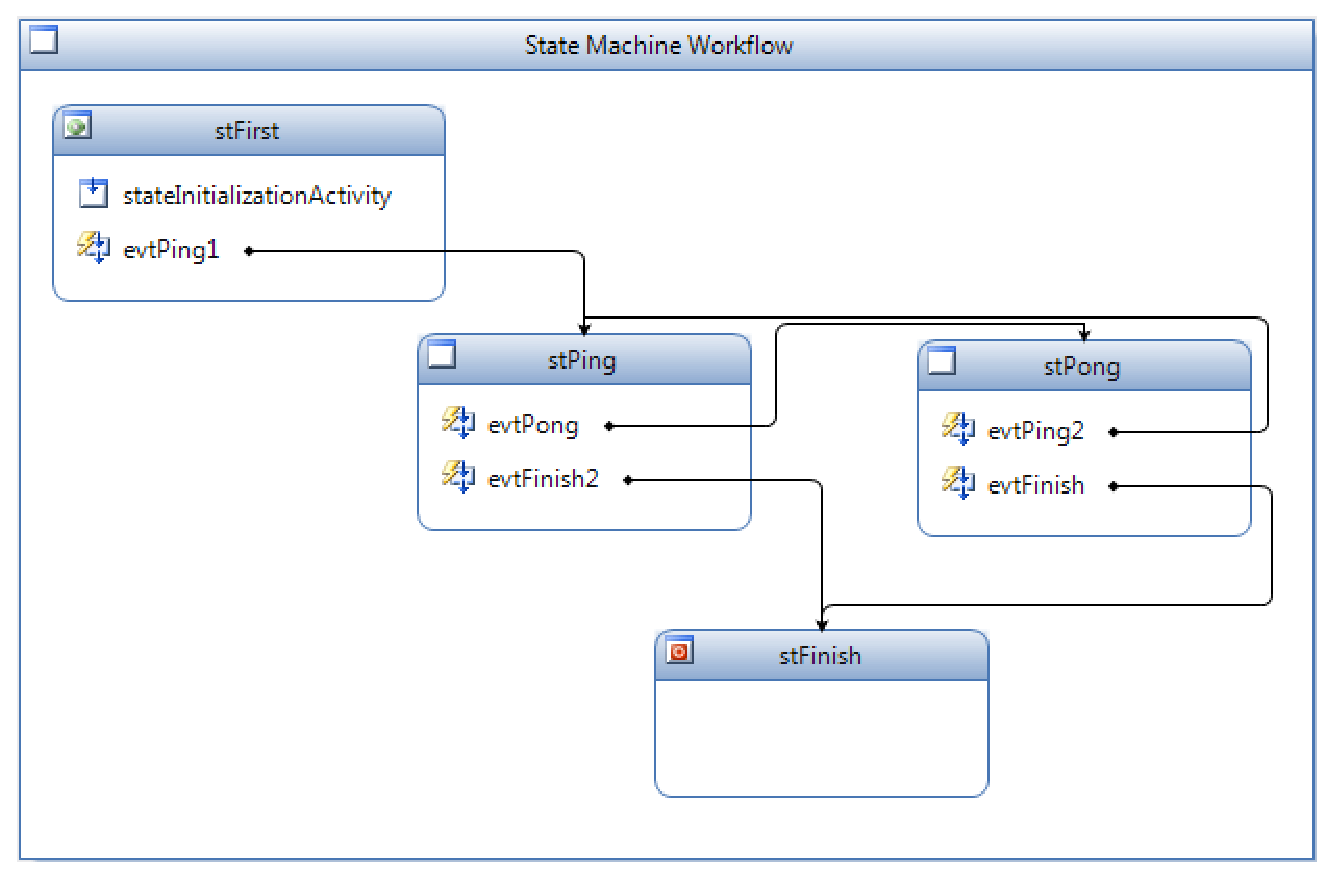
\includegraphics[width=12.22cm,height=7.95cm]{media/image4.eps}
\end{figure}


\begin{center}\textbf{Fig. 4. }: State Machine Implementation
\end{center}



The previously explained interface is exposed to the client side also 
while the implementation of the interface stays on the server side and 
defines properties that are exclusively server specific:

\begin{verbatim}
    [StateMachineParameters(typeof(PingPongWF),  
                          typeof(PingPongController))]
    class PingPongService : MultiSession,   
                                 IPingPongService
    {
...
\end{verbatim}
The StateMachineParameters attribute declares a state machine workflow 
type and a controller type that will be instantiated when the first call 
occurs. This state machine and controller instance will drive the 
process (the game in our example).

\subsection{4.4 Custom Behaviors }
Every call to the exposed operations has to be intercepted on the server 
side and the security checks described in this paper have to be 
performed. WCF has the ability to extend our service endpoints with 
custom behaviors that can be used to do security checks.

We mention that WCF calls do not submit the client side caller type and 
identity information automatically therefore at the client side we have 
to add headers to every call that contain this information using custom 
client-side behaviors.

The following XML fragment shows the server side configuration that 
defines the extension that is responsible for doing security checks 
before the execution of the exposed operation:

\begin{verbatim}
<extensions>
  <behaviorExtensions>
    <add name="distrRac"
         type="ServerLib.RACServerBehaviorExtension, ServerLib, Version=1.0.0.0, Culture=neutral, PublicKeyToken=d18ff0ec0229ce90" />
  </behaviorExtensions>
</extensions>
\end{verbatim}
At the client side, there is a similar configuration setting that refers 
to the ClientLib.RACClientBehaviorExtension type in the ClientLib 
assembly.

Connecting these extensions to the appropriate services some more lines 
of XML configuration has to be added.

We show the client code fragment that adds the type of the caller to the 
request headers that will be verified on the server side:

\begin{verbatim}
StackTrace stackTrace = new StackTrace(false);
StackFrame callerFrame = ClientHelper.GetCallerMethod(stackTrace);
request.Headers.Add(MessageHeader.CreateHeader(
    DISTRRAC_HEADERID, DISTRRAC_NS, 
    callerFrame.GetMethod().DeclaringType.FullName));
\end{verbatim}
On the server side the following code fragment is executed that checks 
the type and identity of the caller:

\begin{verbatim}
string absUri = request.Headers.To.AbsoluteUri;
Type contract = ServerHelper.GetContract(absUri);
object []drivenAttrs = ServerHelper.GetDrivenByAttributes(contract);
MethodInfo targetMethod = ServerHelper.GetTargetMethod(absUri);

bool callerIdentityDriven = 
             ServerHelper.IsDrivenByCallerIdentity(drivenAttrs);
bool stateMachineDriven = 
             ServerHelper.IsDrivenByStateMachine(drivenAttrs);

if (callerIdentityDriven)
{
    object[] callerAttrs = 
           ServerHelper.GetCallerAttributes(targetMethod);
    string callerType = 
           request.Headers.GetHeader<string>(DISTRRAC_HEADERID, 
                                             DISTRRAC_NS);
    if (!ServerHelper.IsCallerAllowed(callerAttrs, callerType))
    {
        throw new InvalidCallerException();
    }
}
\end{verbatim}
The state machine based verification is performed similarly, however, in 
that case after the execution of the exposed operation the state machine 
is driven to the next state.

The other components of the H information set can be checked similarly 
therefore we omit the discussion of their implementation.

\section{5 Related Work}
There are several authors who deal with the security of distributed 
applications and show the importance of the topic $[$2, 21$]$. There are 
techniques which can be used to generate formal proof that an access 
request satisfies an access-control policy $[$3$]$.

$[$6$]$ provides a method for specifying authorization constraints for 
workflow based systems that include separation of duty constraints (two 
different tasks must be executed by different users), binding of duty 
constraints (same user is required to perform multiple tasks) and 
cardinality constraints (specify the number that certain tasks have to 
be executed). A custom reference monitor has been specified that checks 
the previously mentioned properties of workflows and workflow tasks. 

Those parts of our solution that deal with state machines (workflows) 
and client type and identity validation provide some features in a more 
sophisticated way than described in $[$6$]$, however there are some 
features our framework lacks. The difference between the two approaches 
can be characterized by the fact that we are dedicated to find answers 
to shortcomings of working enterprise applications.

The concepts in $[$8$]$ are based on the workflow RBAC authorization 
rules that are represented as a tuple (r, t, execute, p) that states 
that users in r role can execute task t when an optional predicate p 
holds true). They create an extension to the WARM methodology that 
enables to determine workflow access control information from the 
business process model. $[$21$]$ presents an approach where the workflow 
access control model is decoupled from the workflow model that enables 
them to create a service oriented workflow access control model. Our 
solution follows a different approach that makes it more compact but 
harder to configure.

Another way would be to create a DSL that is dedicated to implementing 
services $[$5$]$ and extend this language with security concepts.

There are approaches that store and control policy settings using some 
centralized database $[$7$]$ or have multiple layers of configuration 
$[$18$]$. We decided to create an application specific solution and have 
unified configuration methodology (declaratively specify settings in the 
source text on application level or use application-level configuration 
files).

\section{6 Summary and Future Work}
In this paper we have studied access control mechanisms that can be 
applied in case of distributed software systems.

Applications serving business processes are usually implemented as a 
distributed system: they span over different servers on different 
networks. Typical properties of such applications include dynamism: the 
business goals they serve change just as often as the programming or 
hardware environments. In order to successfully fight challenges imposed 
by the nature of these applications, the basic principles of Service 
Oriented Architecture (SOA) have been formed. SOA is a natural extension 
and descendant of modular programming: the functions of modules are 
published through interfaces.

In our work we have focused on the public interfaces of SOA applications 
with the following restrictions: 

\newcounter{numberedCntBE}
\begin{enumerate}
\item The application should use homogeneous communication platform and 
\item The service should have some information about the clients. 
\setcounter{numberedCntBE}{\theenumi}
\end{enumerate}
We have described motivating examples showing why it is often not enough 
to rely ourselves on standard security mechanisms of existing standards. 
Starting from the motivating examples we have shown why lower level 
access control mechanisms are necessary to protect the interfaces 
exposing functionality to the outside world.

We have elaborated our research and extended the security context of 
distributed applications based on the following properties: distributed 
runtime access control, business process and client identity validation, 
and the network identity validation of clients. The above properties can 
be validated at method level at every single call. The granularity level 
of most of the above properties changes from application level to method 
level. Informally speaking we introduce a business call level 
fine-grained "\,firewall".

We have been following a semi-formal approach of the topic, and have 
given a definition of a legal method call. Other solutions described in 
the related work section solve only a part of the security problems 
specific to distributed enterprise applications while we aimed to create 
a framework that answers most of emerging questions.

The formal approach described important runtime restrictions for 
distributed object systems. However, the formal approach itself cannot 
guarantee that it can be implemented in practice. In order to prove the 
practical applicability of the proposal, we have implemented a pilot 
framework in the .NET 3.0 programming environment. The implementation 
uses the innovative technologies of the .NET framework: Windows 
Communication Foundation and Workflow Foundation. We exploited 
declarative programming to the maximal possible extent.

One of our further research directions can be the extension of the pilot 
implementation with different environments, such as the Java platform. 
The capabilities of widely used industrial standards should be analyzed, 
and, if necessary, the presented formal framework should be refined in 
order to adapt to different security mechanisms.

We designed our framework to be extensible with other custom security 
mechanisms that may be orthogonal to the formalized and implemented 
ones.

This paper also shows the need for runtime access control in order to 
secure distributed applications. Therefore we hope that similar 
frameworks will gain popularity and help the quality improvement of 
complex, distributed object systems.

\section{References}
1. A. Barros, G. Decker, M. Dumas, F. Weber: \textit{Correlation 
Patterns in Service-Oriented Architectures}, In Proceedings of the 
10th International Conference on Fundamental Approaches to Software 
Engineering (FASE 2007), Braga (Portugal), 2007. Springer Verlag, pages 
245-259.

2. M. Blaze, J. Feigenbaum, J. Ioannidis, A. D. Keromytis. \textit{The 
role of trust management in distributed systems security}, Secure 
Internet Programming. Springer Verlag, 1999, pages 185-210

3. L. Bauer, S. Garriss, M. K. Reiter. \textit{Efficient Proving for 
Practical Distributed Access-Control Systems}. Computer Security - 
ESORICS 2007, 2007, Springer Verlag, pages 19-37

4. M. Bicz�, K. P�cza, Z. Porkol�b. \textit{Runtime Access Control in 
C\# 3.0 Using Extension Methods}, Proceedings of the 10th Symposium on 
Programming Languages and Software Tools (SPLST 2007), Dobog�k� 
(Hungary), 2007, pages 45-60.

5. D. Cooney, M. Dumas, P. Roe: \textit{GPSL:} \textit{A Programming 
Language for Service Implementation}, In Proceedings of the 8th 
International Conference on Fundamental Approaches to Software 
Engineering (FASE), Vienna, Austria, March 2006. Springer Verlag, pages 
3-17.

6. J. Crampton: \textit{A reference monitor for workflow systems with 
constrained task execution}, In Proceedings of the 10th ACM Symposium 
on Access Control Models and Technologies, pages 38-47, 2005.

7. N. Damianou, N. Dulay, E. Lupu, M. Sloman and T. Tonouchi. \textit{
Policy Tools for Domain Based Distributed Systems Management}. 
IFIP/IEEE Symposium on Network Operations and Management. Florence, 
Italy, 2002.

8. D. Domingos, A. R. Silva, P. Veiga. \textit{Workflow Access Control 
from a Business Perspective}. International Conference on Enterprise 
Information Systems, 2004

9. Frank E. Developing Distributed Enterprise Applications With the MS 
Common Object Model. Hungry Minds, 1997, ISBN 0-764580-44-2

10. R. Gronmo, M. C. Jaeger, A. Wombacher: \textit{A Service 
Composition Construct to Support Iterative Development}, In 
Proceedings of the 10th International Conference on Fundamental 
Approaches to Software Engineering (FASE 2007), Braga (Portugal), 2007. 
Springer Verlag, pages 230-244.

11. M. B. Juric, B. Mathew, P. Sarang. \textit{Business Process 
Execution Language for Web Services: BPEL and BPEL4WS}, Packt 
Publishing, 2004, ISBN 1-904811-18-3

12. G. Kiczales, J. Lamping, A. Mendhekar, C. Maeda, C. Lopes, J.-M. 
Loingtier, J. Irwin. \textit{Aspect-Oriented Programming}, 
Proceedings of the European Conference on Object-Oriented Programming, 
1997, Springer Verlag, pages 220-242.

13. B. Meyer. Eiffel - The Language, Prentice Hall, 1992. ISBN 
0-13-247925-7

14. .NET Framework: http://msdn2.microsoft.com/netframework/

15. K. P�cza, M. Bicz�, Z. Porkol�b. \textit{Runtime Access Control in 
C\#}, Proceedings of the 7th International Conference on Applied 
Informatics (ICAI), Eger, Hungary, 2007, jan. 28-31.

16. A. Snyder. \textit{Encapsulation and inheritance in object-oriented 
programming languages}. In Proceedings of OOPSLA '86, pages 38-45. ACM 
Press, 1986.

17. Z. Tari, O. Bukhres. \textit{Fundamentals of Distributed Object 
Systems: The CORBA Perspective}, Wiley, 2001, ISBN 978-0-471-35198-6

18. D. Thomsen, D. O'Brien, and J. Bogle. \textit{Role Based Access 
Control Framework for Network Enterprises}. In Proceedings of 14th 
Annual Computer Security Applications Conference. December 1998

19. UML: http://www.uml.org/

20. S. Weerawarana, F. Curbera, F. Leymann, T. Storey, D. F. Ferguson. 
\textit{Web Services Platform Architecture : SOAP, WSDL, WS-Policy, 
WS-Addressing, WS-BPEL, WS-Reliable Messaging, and More}. Prentice 
Hall PTR, 2005.

21. X. Wei, W. Jun, L. Yu, L. Jing. \textit{SOWAC: a service-oriented 
workflow access control model}. Proceedings of the 28th Annual 
International Computer Security and Applications Conferences, 2004, 
pages 128-134.

22. Windows Communication Foundation: http://wcf.netfx3.com/

23. Windows Workflow Foundation: http://wf.netfx3.com/

\end{document}
